\section{HEC-RAS Unsteady}
%%%%%%%%%%%%%%%%%%%%%%%%%%%
what is HEC-RAS?
what is unsteady?

\subsection{Examples}

\subsubsection{Example 3 -- Sudden Gate Closing in an Aqueduct Channel}
Flow in a 1000-m long trapezoidal channel with a bottom width of 20-m, side slope of 2H:1V, longitudinal slope $S_0$=0.0001, and Manning's resistance n=0.013. 
Initial discharge in the channel is 110 m3/s and initial flow depth is 3.069 m.
Simulate the flow and depth at every 100-m station when a downstream gate is closed at t=0. 
Produce a graph of depth and velocity versus location for t=0, 60, 360 seconds.\footnote{Example 12-1, Page 623. Roberson, J A., Cassidy, J.J., and Chaudhry, M. H. (1988). Hydraulic Engineering. Houghton Mifflin Co., Boston, 662p. }

\subsubsection{Example 4 -- Flood Hydrograph in Horizontal Channel}
The initial depth in a 5 meter wide horizontal channel of rectangular cross section is 1 meter. 
The channel is 29 kilometers long and ends with a non-reflection boundary condition.

\begin{figure}[h!] %  figure placement: here, top, bottom, or page
   \centering
   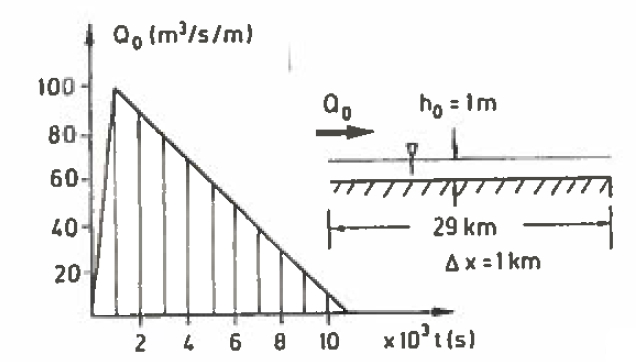
\includegraphics[width=4.0in]{upstreamHydro.jpg} 
   \caption{Upstream hydrograph for example}
   \label{fig:upstreamHydro}
\end{figure}

The initial discharge in the channel is 0 cubic meters per second. 
The upstream input hydrograph is shown in Figure \ref{fig:upstreamHydro}.
The manning friction factor is $n=1/40$.
Simulate the water surface elevation over time in the channel.\footnote{Modified from Example 4.1, Page 70. Koutitas, C.G. (1983). Elements of Computational Hydraulics. Pentech Press, London 138p. ISBN 0-7273-0503-4 }

\begin{figure}[h!] %  figure placement: here, top, bottom, or page
   \centering
   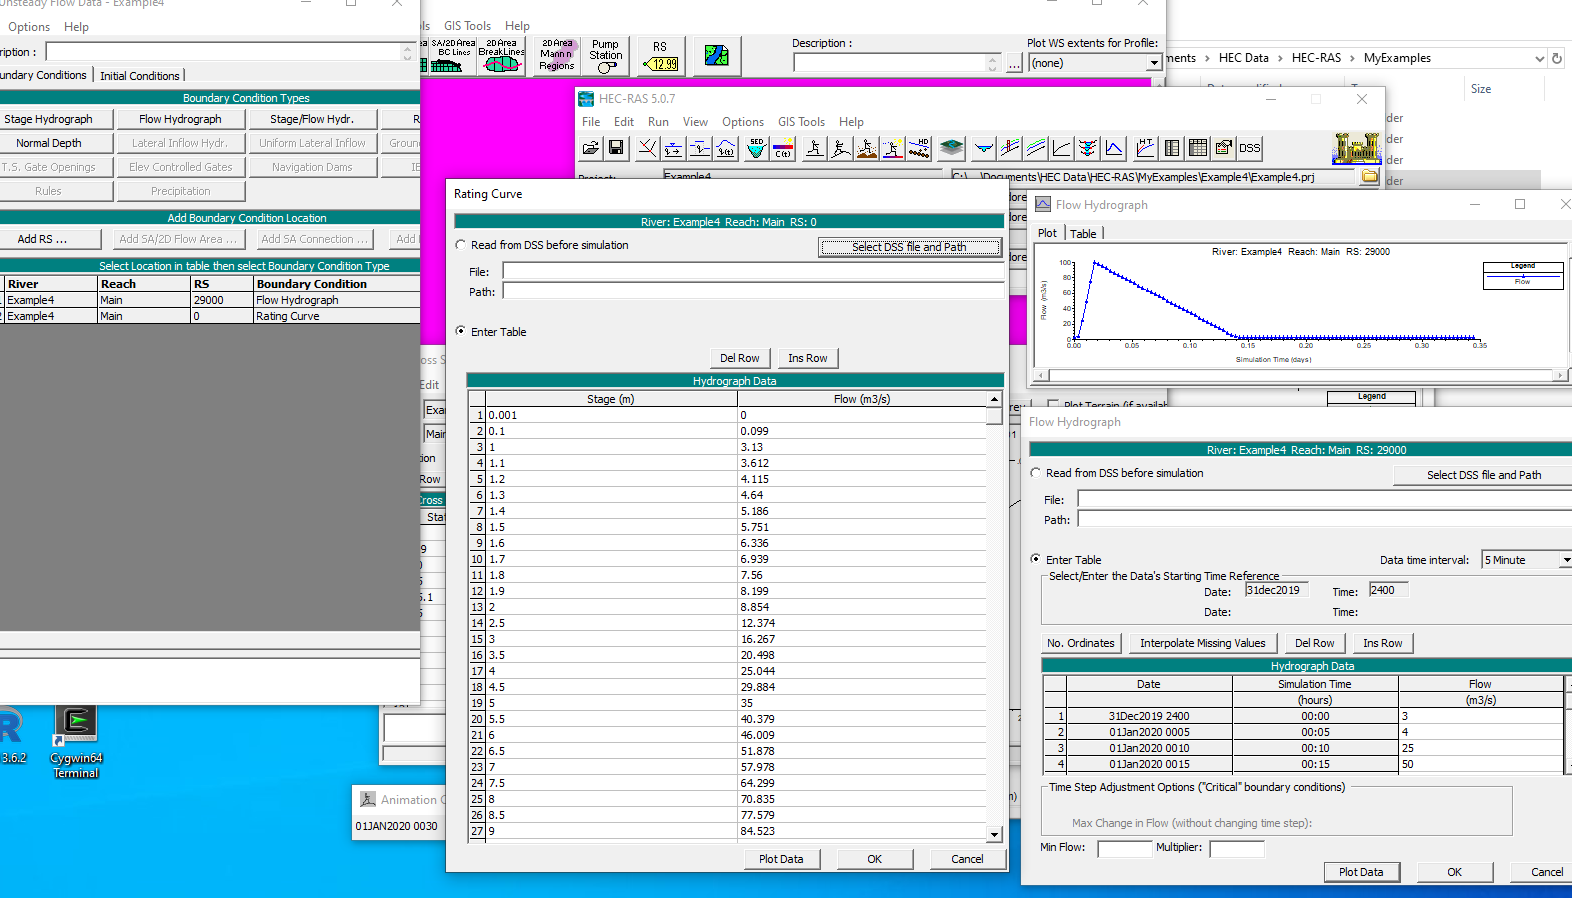
\includegraphics[width=4.25in]{ex4bc.png} 
   \caption{Boundary conditions -- Upstream is time-varying flow; Downstream is a rating curve (depth vs flow) if depth is critical, then simulating a free outfall}
   \label{fig:ex5bc}
\end{figure}

\begin{figure}[h!] %  figure placement: here, top, bottom, or page
   \centering
   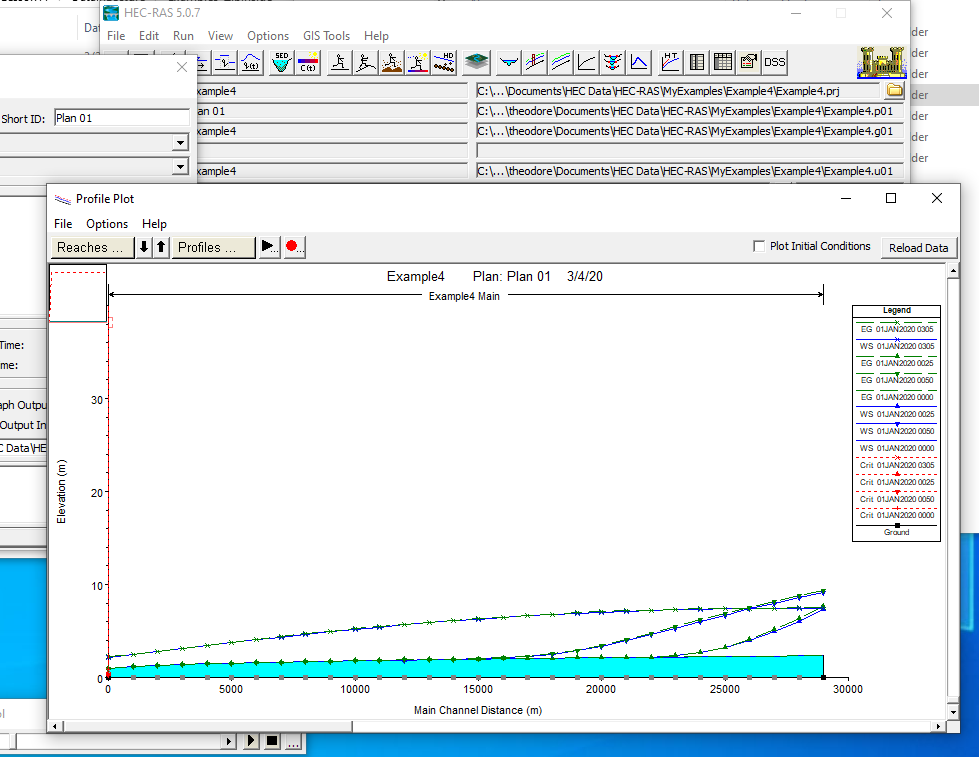
\includegraphics[width=4.25in]{ex4wsp.png} 
   \caption{WSP at several times -- flood wave is apparent.}
   \label{fig:ex5wsp}
\end{figure}

\subsubsection{Example 5 -- Long waves in a Tidal-Influenced Channel}
Simulate the propogation of a long wave of period T=600sec (10 minutes) along an estuary of rectangular cross section bottom slope 0.4\% and friction coefficient $n=\frac{1}{30}$.
The amplitude of the tide at the open sea boundary is 3 meters.\footnote{Example 4.2, Page 77. Koutitas, C.G. (1983). Elements of Computational Hydraulics. Pentech Press, London 138p. ISBN 0-7273-0503-4 }

\begin{figure}[h!] %  figure placement: here, top, bottom, or page
   \centering
   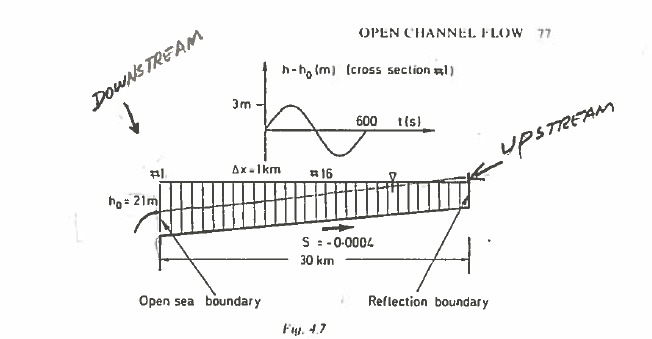
\includegraphics[width=4.25in]{ex5scheme.png} 
   \caption{Schematic --- Long Waves in Open Channel}
   \label{fig:ex5scheme}
\end{figure}

What is the depth and water velocity at 15 km from the open boundary?

\begin{figure}[h!] %  figure placement: here, top, bottom, or page
   \centering
   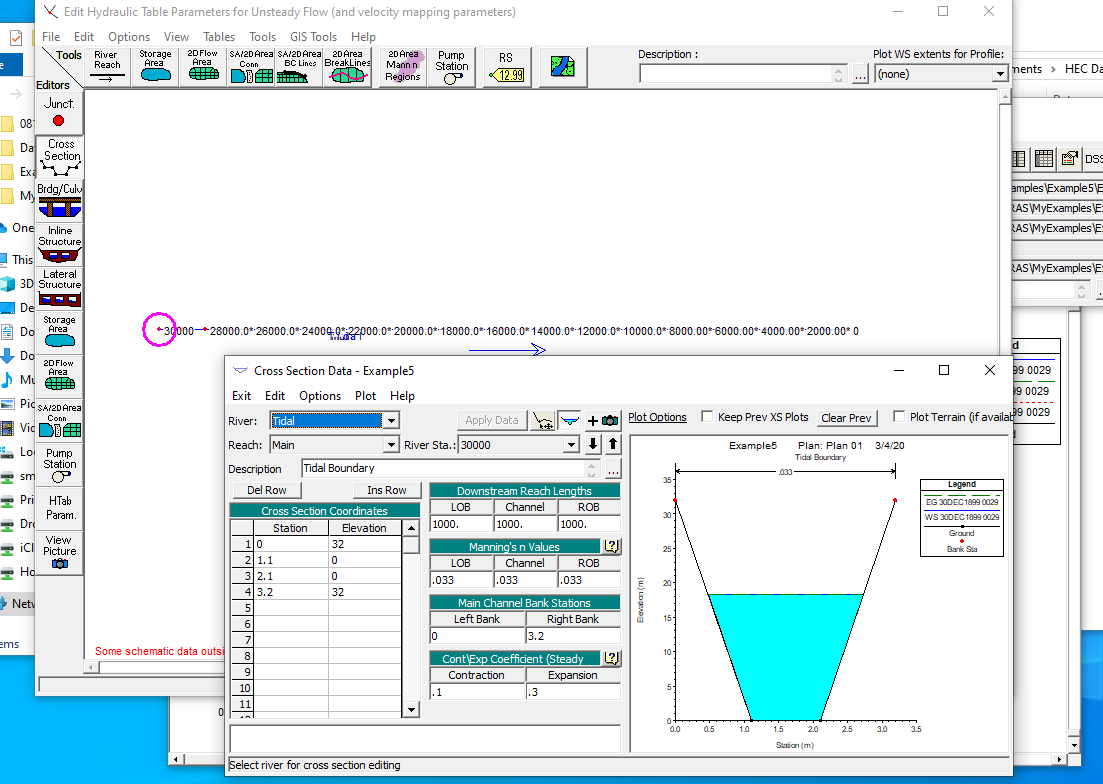
\includegraphics[width=4.25in]{ex5geom.png} 
   \caption{Geometry -- the "trapezoid" has steep side walls and graphic is deceptive}
   \label{fig:ex5geom}
\end{figure}

\begin{figure}[h!] %  figure placement: here, top, bottom, or page
   \centering
   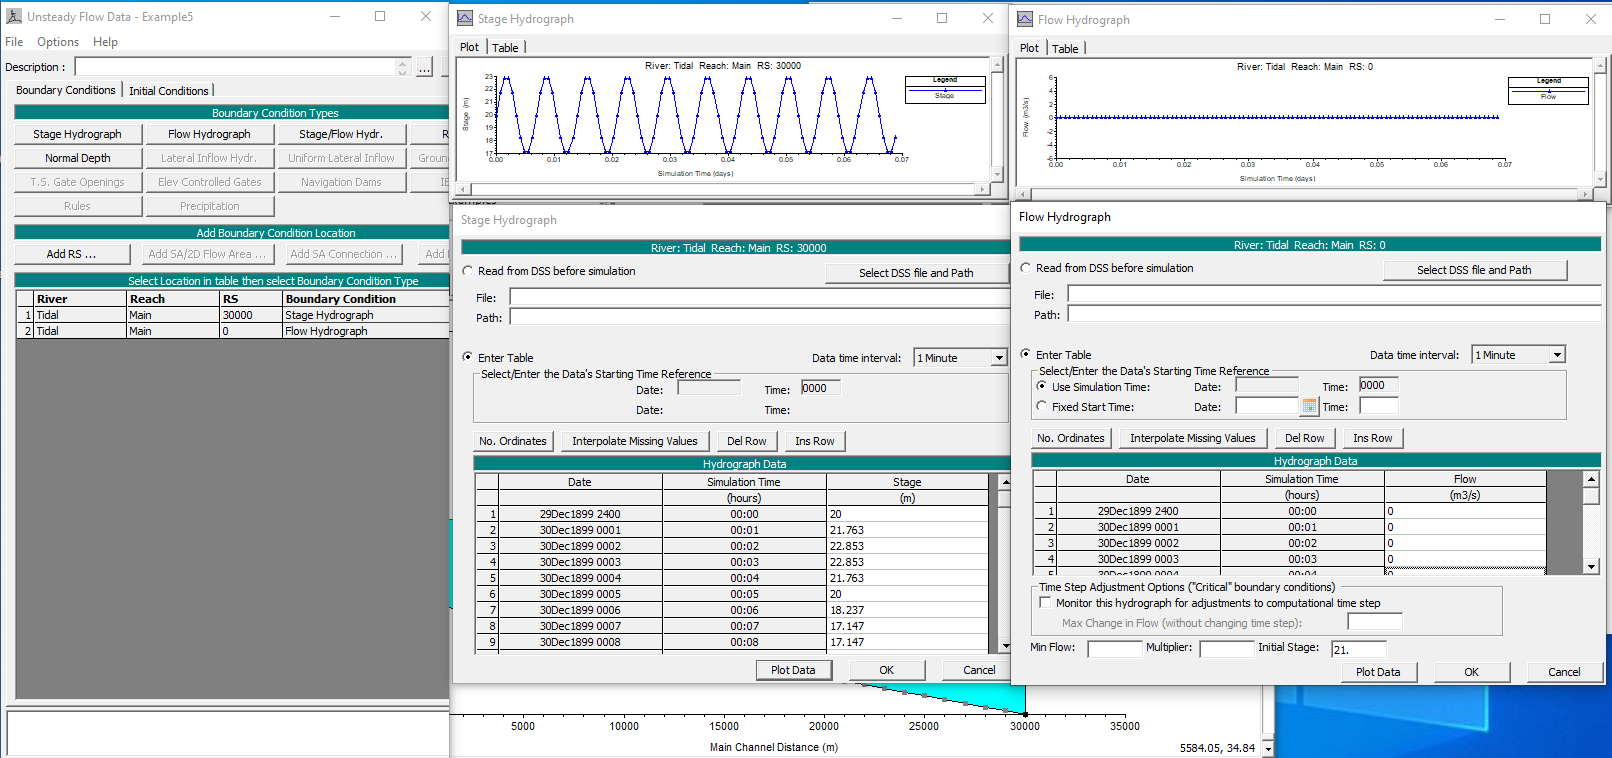
\includegraphics[width=4.25in]{ex5bc.png} 
   \caption{Boundary conditions -- Upstream is time-varying stage; Downstream is fixed zero discharge (should reflect incoming waves)}
   \label{fig:ex5bc}
\end{figure}

\begin{figure}[h!] %  figure placement: here, top, bottom, or page
   \centering
   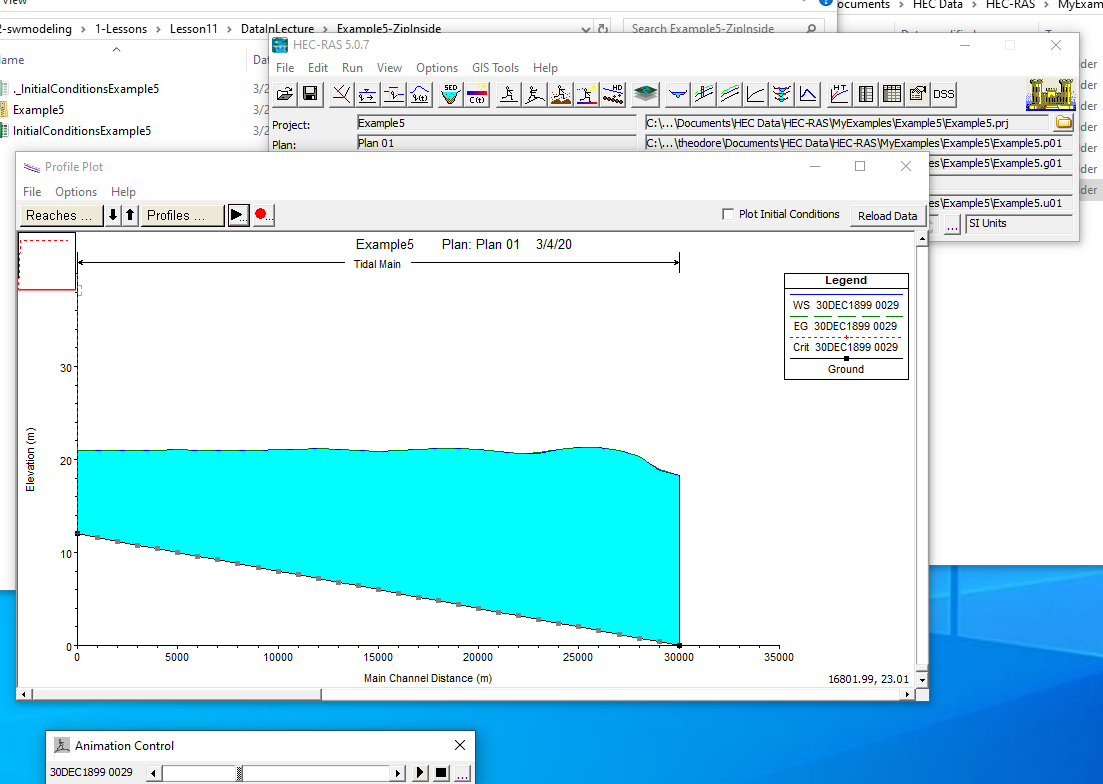
\includegraphics[width=4.25in]{ex5wsp.png} 
   \caption{WSP at some time slice}
   \label{fig:ex5wsp}
\end{figure}

\subsection{Appendix}
